\documentclass[]{article}
\usepackage{amsmath}
\usepackage[margin=0.7in]{geometry}
\usepackage{graphicx}
\usepackage{grffile}
\usepackage{graphics}
\usepackage{amssymb}% http://ctan.org/pkg/amssymb
\usepackage{pifont}% http://ctan.org/pkg/pifont
\newcommand{\cmark}{\ding{51}}%
\newcommand{\xmark}{\ding{55}}%
%opening
\title{NWEN242 Assignment 4}
\author{Vincent Yu || 300390526}

\begin{document}

\maketitle
\section*{Q1}
\subsection*{a}
It can store 4 Integers.\newline
32-bit =4- byte\newline
$\dfrac{16}{4}$=4\newline
Hence it can store four integers.\newline
\subsection*{b}
The variables i and j are accessed through each iteration. I and J exhibits temporal locality in the inner loop function. We also use B[I][0] through each iteration. Hence B[I][0] also exhibits temporal locality.\newline 
\subsection*{c}
A[I][J] exhibits spatial locality. Because in the inner loop J changes through each iteration and the value placed next to each other, once J reaches 7999 it will start again from 0. \newline


\section*{Q2}
\subsection*{a}
\begin{center}
	\begin{tabular}{ c c c c c   }
		Word Address & Binary Address & Tag & Index & Hit/Miss\\
		3 & 0000 0011 &  0 & 3 & M\\
		180 & 1011 0100 & 11 & 4 & M\\
		43 & 0010 1011 & 2 & 11 & M\\
		2 & 0000 0010 & 0 & 2 & M\\
		191 & 1011 1111 & 11 & 15 & M\\
		88 & 0101 1000 & 5 & 8 & M\\
		190 & 1011 1110 & 11 & 14 & M\\
		14 & 0000 1110 & 0 & 14 & M\\
		181 & 1011 0101 & 11 & 5 & M\\
		44 & 0010 1100 & 2 & 12 & M\\
		186 & 1011 1010 & 11 & 10 & M\\
		253 & 1111 1101 & 15 & 13 & M\\
	\end{tabular}
\end{center}

\subsection*{b}
\begin{center}
	\begin{tabular}{ c c c c c   }
		Word Address & Binary Address & Tag & Index & Hit/Miss\\
		3 & 0000 0011 &  0 & 1 & M\\
		180 & 1011 0100 & 11 & 2 & M\\
		43 & 0010 1011 & 2 & 5 & M\\
		2 & 0000 0010 & 0 & 1 & H\\
		191 & 1011 1111 & 11 & 7 & M\\
		88 & 0101 1000 & 5 & 4 & M\\
		190 & 1011 1110 & 11 & 7 & H\\
		14 & 0000 1110 & 0 & 7 & M\\
		181 & 1011 0101 & 11 & 2 & H\\
		44 & 0010 1100 & 2 & 6 & M\\
		186 & 1011 1010 & 11 & 5 & M\\
		253 & 1111 1101 & 15 & 6 & M\\
	\end{tabular}
\end{center}
\subsection*{c}
\begin{center}
	\begin{tabular}{ c c c c c c c c c   }
		&&&Cache1 &&Cache2&&Cache3\\
		Word Address & Binary Address & Tag & Index & Hit/Miss & Index &Hit/Miss &Index & Hit/Miss \\
		3 & 0000 0011 & 0 & 3 & M & 1 & M & 0 & M \\
		180 & 1011 0100 & 22 & 4 & M & 2 & M & 1 & M \\
		43 & 0010 1011 & 5 & 3 & M & 1 & M & 0 & M \\
		2 & 0000 0010 & 0 & 2 & M & 1 & M & 0 & M\\
		191 & 1011 1111 & 23 & 7 & M & 3 & M &1 & M \\ 
		88 & 0101 1000 & 11 & 0 & M & 0 & M & 0 & M \\ 
		190 & 1011 1110 & 23 & 6 & M & 3 & H & 1 & H\\ 
 		14 & 0000 1110 & 1 & 6 & M & 3 & M & 1 & M\\ 
		181 & 1011 0101 & 22 & 5 & M & 2 & H & 1 & M\\ 
		44 & 0010 1100 & 5 & 4 & M & 2 & M & 1 & M\\ 
		186 & 1011 1010 & 23 & 2 & M & 1 & M & 0 & M\\ 
		253 & 1111 1101 & 31 & 5 & M & 2 & M & 1 & M\\
	\end{tabular}
\end{center}
Cache 1 : \newline
Miss Rate: 100\% \newline
Total Cycle : 12 $\times$ 25 +12 $\times$ 2 =324 \newline
Cache 2 : \newline
Miss Rate : $\dfrac{10}{12}$ $\approx$ 83\%\newline
Total Cycle: 10 $\times$  25+ 12 $\times$ 3 =286\newline
Cache 3 : 
Miss Rate:  $\dfrac{10}{12}$ $\approx$ 92\% \newline
Total Cycle : 11 $\times$ 25 + 12 $\times$ 5 = 335\newline
From the information shown above, cache2 provides the best performance.
\subsection*{d}
Cache Data Size : 32 KiB\newline
Cache Block Size : 2 words\newline
block numbers= $\dfrac{2^{15}}{2^3}$ = $2^{12}$\newline
(Note: here I divide three because each word have 2 byte and the cache is 2-word cache, it can hold 2 words per block so I divide it by 2 again. In order to find how many blocks we have. )\newline
So the index is 12 bits to identify each block.\newline
Because of 2 words block, the offset is 1 bit.\newline
Tag = 32 - index - offset = 32 - 12 - 1 = 19 bits\newline
Total block size : 1 + 19 + 64 = 84 bits\newline
Total cache size : $\dfrac{84 \times 2^{12}}{8\times 1024}\approx$ 42 KiB \newline

\section*{Q3}
\subsection*{a}
The cache block size = $2^{5}$=32 bytes \newline
In words : $\dfrac{32}{4}$=8\newline
\subsection*{b}
From the 5-bits index, it shows the cache has 32 blocks($2^5$=32).
\subsection*{c}
For each block it has 8 words (8 $\times$ 4=32 bytes), 32 $\times$ 8 =256-bits \newline
Data storage : 32 $\times$ 256 = 8192 bits\newline
Total storage: (256 + 22 + 1) $\times$ 32 = 8928 bits\newline
The ratio is $\dfrac{8298}{8192}$= 1.089\newline
\section*{Q5}
From three way associative cache, it determines we have a 8 sets cache. So the index is 3 bits. Because the cache we have is a two-word cache so the less significant bit is the offset. 
\begin{center}
	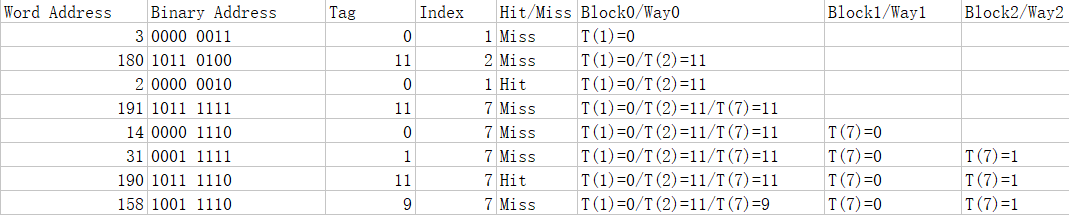
\includegraphics[width=150mm]{n242.png}
\end{center}
\end{document}